\chapter{Made in France} 
\label{sec:mif}
\lstset{style=6502Style}
\begin{figure}[H]
    \centering
      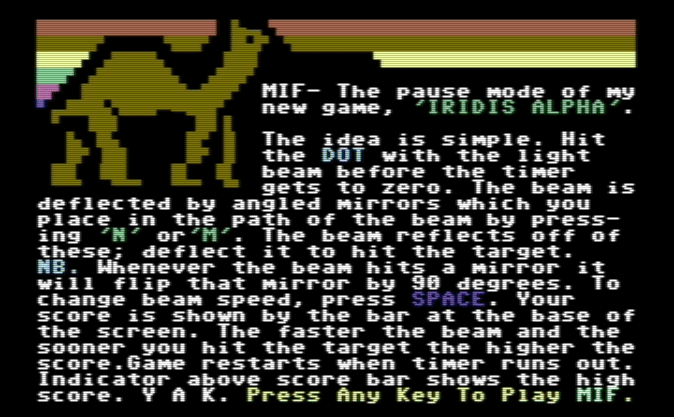
\includegraphics[width=10cm]{src/mif/mif.png}%
\caption{Splash screen\index{screen} for the version of 'Made in France' released on Compunet.}
\end{figure}

I must admit I don't find this pause-mode mini-game of much interest in its own right. I initially
wondered if Jeff Minter had inadvertently invented a precursor to 'Snake', a text-based game that
was once ubiqitous thanks to its inclusion on Nokia mobile phones in the 1990s, but it turns out that
Snake dates back to at least 1976 when the concept first appeared in an arcade game called 'Blockade'.
\begin{figure}[H]
  {
    \setlength{\tabcolsep}{3.0pt}
    \setlength\cmidrulewidth{\heavyrulewidth} % Make cmidrule = 
	\centering
	\begin{subfigure}{0.5\textwidth}
    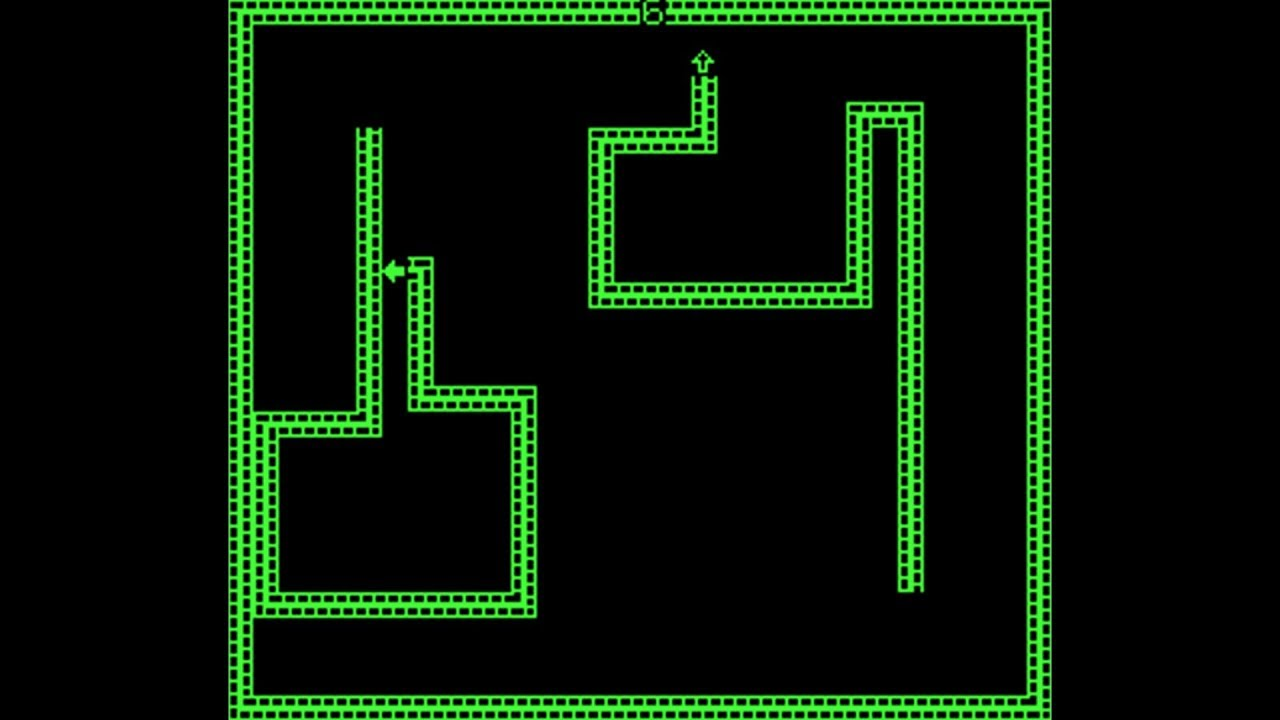
\includegraphics[width=6cm]{src/mif/blockade.jpg}%
	\end{subfigure}
	\begin{subfigure}{0.5\textwidth}
      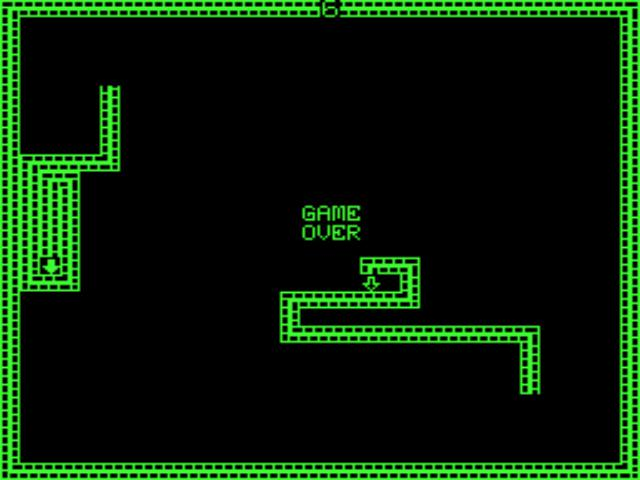
\includegraphics[width=6cm]{src/mif/blockade2.jpg}%
	\end{subfigure}
  }

\caption{'Blockade' from 1976, a two-player arcade game by Gremlin.}
\end{figure}

Perhaps the most noteworthy thing about 'Made in France' (MIF) is how many times Minter has made and remade it. His very
first attempt at the format was one of his earliest games. 'Deflex' was coded in 1979 while he was in Queen Mary's Sixth Form college
in Basingstoke and had access to a 
Commodore PET. Viewed side by side it's obvious that one is a slightly more colorful
remake of the other.

\begin{figure}[H]
  {
    \setlength{\tabcolsep}{3.0pt}
    \setlength\cmidrulewidth{\heavyrulewidth} % Make cmidrule = 
	\centering
	\begin{subfigure}{0.5\textwidth}
    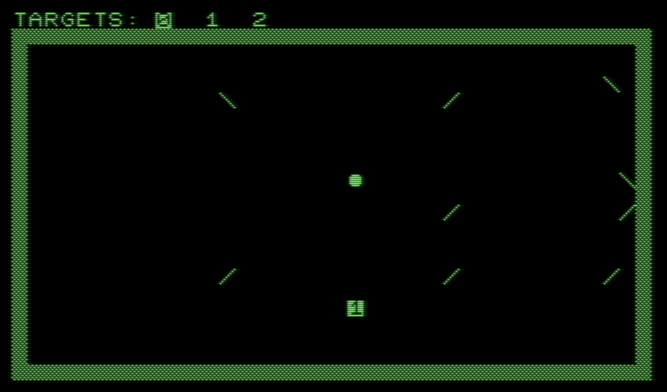
\includegraphics[width=6cm]{src/mif/deflex.png}%
	\end{subfigure}
	\begin{subfigure}{0.5\textwidth}
      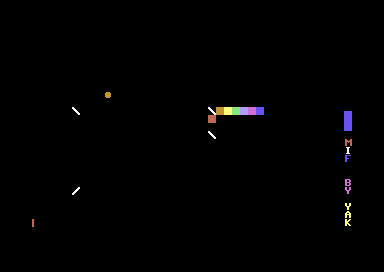
\includegraphics[width=6cm]{src/mif/mif_game.png}%
	\end{subfigure}
  }

\caption{'Deflex' on the left, 'Made in France' on the right. The original Commodor PET version of 'Deflex' is lost, so in 2023 
  \href{https://archive.org/details/deflex-remake}{\textcolor{blue}{Jeff Minter remade it!}}}
\end{figure}

`Made in France' (or MIF for short) was coded while on a winter holiday in France during the making of Iridis Alpha. Minter lugged his development kit to
a ski resort in the Alps and continued work between time on the slopes. Over a couple of spare evenings he remade Deflex into
MIF. He shared this version on Compunet prior to the release of Iridis Alpha and the version that features in the game is unchanged
from that original version.

The gameplay of Deflex and MIF has only a couple of differences. In MIF the player is on a timer and dies if they fail to
complete the level before it elapses.

\begin{figure}[H]
  {
    \setlength{\tabcolsep}{3.0pt}
    \setlength\cmidrulewidth{\heavyrulewidth} % Make cmidrule = 
	\centering
	\begin{subfigure}{0.5\textwidth}
      \frame{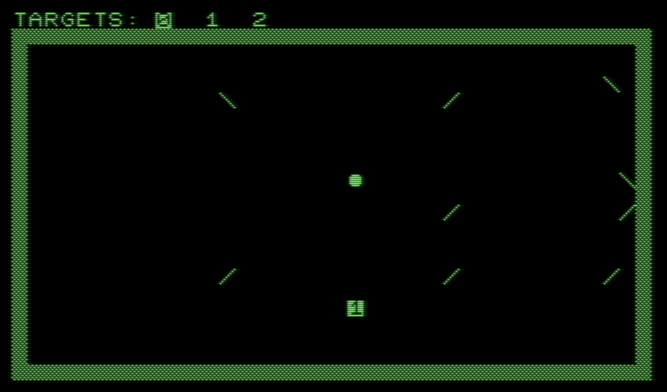
\includegraphics[width=6cm]{src/mif/deflex.png}}
	\end{subfigure}
	\begin{subfigure}{0.5\textwidth}
      \frame{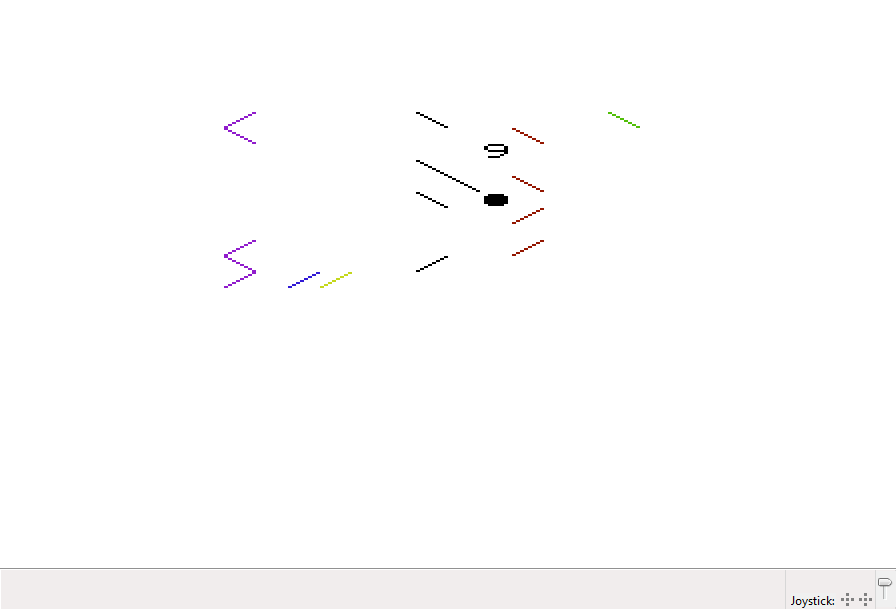
\includegraphics[width=6cm]{src/mif/DeflexV_VIC20.png}}
	\end{subfigure}
	\begin{subfigure}{0.5\textwidth}
  \vspace{0.3cm}
      \frame{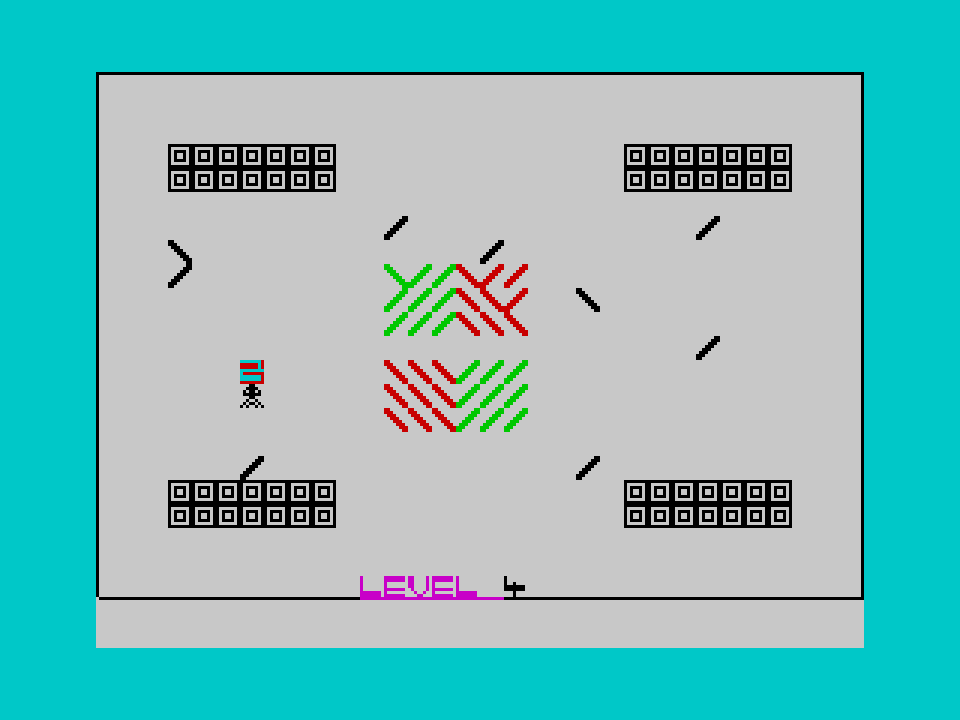
\includegraphics[width=6cm]{src/mif/SuperDeflex_ZXSpectrum.png}}
	\end{subfigure}
	\begin{subfigure}{0.5\textwidth}
  \vspace{0.3cm}
      \frame{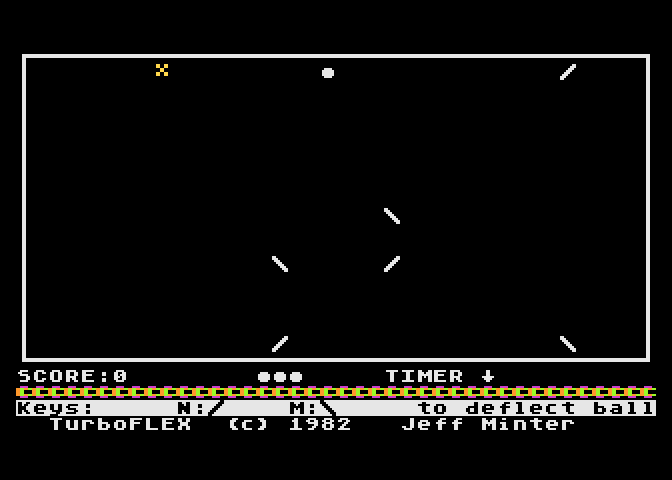
\includegraphics[width=6cm]{src/mif/TurboFlexAtari.png}}
	\end{subfigure}
	\begin{subfigure}{0.5\textwidth}
  \vspace{0.3cm}
      \frame{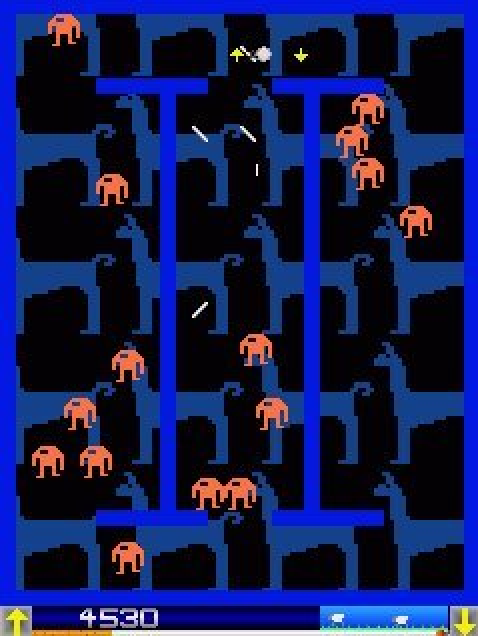
\includegraphics[width=6cm]{src/mif/Deflex_PocketPC.png}}
	\end{subfigure}
	\begin{subfigure}{0.5\textwidth}
  \vspace{0.3cm}
      \frame{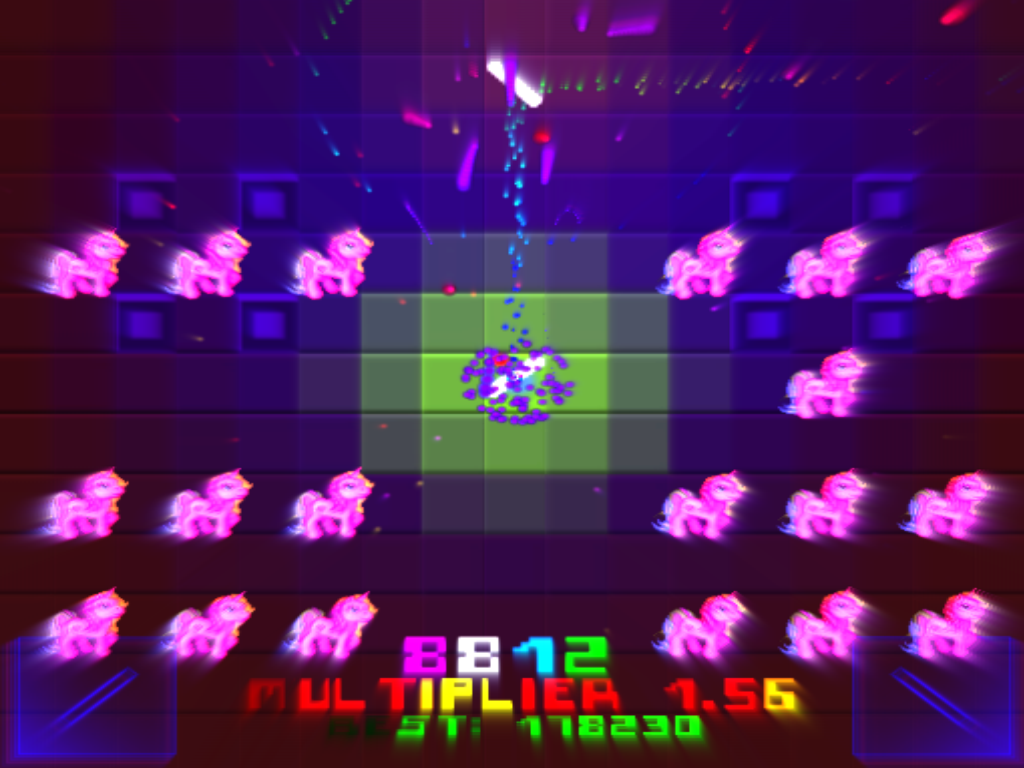
\includegraphics[width=6cm]{src/mif/Deflex_IOS.png}}
	\end{subfigure}
  }
\caption{Deflex through the ages. }
\end{figure}
\clearpage

The most striking thing to the modern player is the controls. You place paddles (or deflectors) by using the 'N' and 'M' keys. At first
this seems inexplicable: why not use arrow keys instead? The answer lies in the layout of the C64 and Commodore Pet keyboards: 
\begin{figure}[H]
  {
    \setlength{\tabcolsep}{3.0pt}
    \setlength\cmidrulewidth{\heavyrulewidth} % Make cmidrule = 
	\centering
	\begin{subfigure}{0.5\textwidth}
    \frame{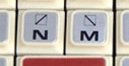
\includegraphics[width=6cm]{src/mif/pet_nm.jpg}}
	\end{subfigure}
	\begin{subfigure}{0.5\textwidth}
    \frame{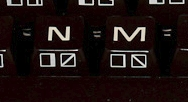
\includegraphics[width=6cm]{src/mif/c64_nm.jpg}}
	\end{subfigure}
  }
\caption{ The controls seem unintuitive to a player using a C64 emulator. Why use 'M' and 'N' for placing paddles? The answer lies in the PET
and C64 keyboard\index{keyboard} layouts: the 'm' and 'n' keys each bear the paddle glyphs.
}
\end{figure}

\subsubsection{Main Loop}
The code for MIF comes in at a relatively light 900 or so lines of 6502
assembler. The main loop of the game is primarily concerned with detecting key
presses to enter into the DNA mini-game (see
\hyperref[sec:dna]{\textcolor{blue}{A Pause Mode for Your Pause Mode}}) or exit
back to Iridis Alpha itself.

\begin{lstlisting}[escapechar=\%]
MIF_RunUntilPlayerUnpauses%\index{MIF\_RunUntilPlayerUnpauses}%   
    JSR MIF_InitializeProgressBar%\index{MIF\_InitializeProgressBar}%
    JSR MIF_DrawCountdownBarAndCredit%\index{MIF\_DrawCountdownBarAndCredit}%
    JSR MIF_UpdateProgressBar%\index{MIF\_UpdateProgressBar}%
    JSR MIF_SetUpInterruptHandler%\index{MIF\_SetUpInterruptHandler}%
MIF_MainLoop%\index{MIF\_MainLoop}%
    LDA lastKeyPressed%\index{lastKeyPressed}%
    CMP #$40 ; 'No key pressed'
    BNE MIF_MainLoop%\index{MIF\_MainLoop}%

    LDA #$00
    STA $D015    ;Sprite display Enable

    ; Maybe Exit Back to Game
MaybeExitBackToGame
    LDA lastKeyPressed%\index{lastKeyPressed}%
    CMP #$04 ; F1
    BNE MaybeAsteriskPressed
    ;F1 was pressed, so exit MIF back to game.
    RTS 

MaybeAsteriskPressed
    CMP #$31; '*' Pressed
    BNE MaybeLaunchNewGame

    ; If '*' was pressed, launch DNA.
MIF_DoubleCheckKeyPress%\index{MIF\_DoubleCheckKeyPress}%
    LDA lastKeyPressed%\index{lastKeyPressed}%
    CMP #$40 ; 'No key pressed'
    BNE MIF_DoubleCheckKeyPress%\index{MIF\_DoubleCheckKeyPress}%

    ; Launch DNA
    LDA #$01
    STA mifDNAPauseModeActive%\index{mifDNAPauseModeActive}%
    JSR EnterMainTitleScreen%\index{EnterMainTitleScreen}%

    ; Relaunch MIF when player exits DNA.
    JMP LaunchMIF%\index{LaunchMIF}%

MaybeLaunchNewGame
    LDA mifGameOver%\index{mifGameOver}%
    BEQ MaybeExitBackToGame
    JMP LaunchMIF%\index{LaunchMIF}%
\end{lstlisting}

The actual gameplay is handled from an interrupt\index{interrupt} once per frame.

\begin{lstlisting}[escapechar=\%]
MIF_InterruptHandler%\index{MIF\_InterruptHandler}%   
    LDA $D019    ;VIC Interrupt%\index{Interrupt}% Request Register%\index{Register}% (IRR)
    AND #$01
    ; Limits the updates to once per frame.
    BNE PerformGamePlayUpdates
    PLA 
    TAY 
    PLA 
    TAX 
    PLA 
    RTI 

PerformGamePlayUpdates
    JSR UpdateSnakePositionAndCheckInput%\index{UpdateSnakePositionAndCheckInput}%
    JSR MIF_UpdateCountdownBar%\index{MIF\_UpdateCountdownBar}%
    JSR MIF_PlaySound%\index{MIF\_PlaySound}%
    JSR MIF_UpdateTarget%\index{MIF\_UpdateTarget}%
    LDA #$01
    STA $D019    ;VIC Interrupt%\index{Interrupt}% Request Register%\index{Register}% (IRR)
    STA $D01A    ;VIC Interrupt%\index{Interrupt}% Mask Register%\index{Register}% (IMR)
    LDA #$FE
    STA $D012    ;Raster Position
    JMP $EA31
\end{lstlisting}

\subsubsection{A Target Explodes}
One point of interest in this mini-game is the explosion when you finally overcome the
frustrating controls and manage to strike the target with your snake.
\begin{figure}[H]
    \centering
    \foreach \l in {1, ..., 6}
    {
      \begin{subfigure}{0.3\textwidth}
      \includegraphics[width=3cm]{mif/explosion/\l-crop.png}%
      \end{subfigure}
    }%
\caption{Stages in the target's explosion}
\end{figure}

If we carefully examine the sequence of the explosion above it is possible to discern what
is going on. At each step we paint eight red squares. In the first step, these eight squares will
enclose our target giving us a solid block. 
\begin{figure}[H]
    \centering
      \frame{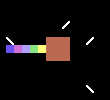
\includegraphics[width=3cm]{mif/explosion/1-crop.png}}%
\caption{Step One}
\end{figure}

In the following step, we paint eight red squares again but this time we separate each with a single space.
We also paint eight squares again like we did in the first step, but this time in the colour brown.
\begin{figure}[H]
    \centering
      \frame{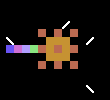
\includegraphics[width=3cm]{mif/explosion/2-crop.png}}%
\caption{Step Two}
\end{figure}

In the third step, we paint eight red squares again but this time we separate each with two spaces.
We also paint eight squares separated by a single space, but this time in the color brown.
Finally we paint eight sqaures separated by no spaces and this time in the colour yellow.
\begin{figure}[H]
    \centering
      \frame{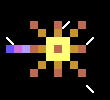
\includegraphics[width=3cm]{mif/explosion/3-crop.png}}%
\caption{Step Three}
\end{figure}

Are you beginning to get the idea? We do this until we have used up all 8 colours and we keep exploding
until we have reached a limit of 48 spaces between squares. 

Here is the routine that runs every time the
interrupt is called and there's an explosion in progress. It maintains the current outer limit of the 
explosion in \icode{previousSpacesBetweenSquares} and works inwards each time it is called, painting the
layers of the explosion in ever-decreasing circles:

\begin{lstlisting}[escapechar=\%, caption=The routine responsible for animating a frame of the explosion\, it will
keep getting called until it sets \icode{targetIsExploding} to \icode{\$00}.]
DoAnExplosionFrame
		    LDA #$A0
        STA mifCurrentChar
        LDA previousSpacesBetweenSquares
        STA spacesBetweenSquares
        LDA #$00
        STA currentColor

PopulateAStageInTheExplosionLoop   
        JSR PopulateAStageInTheExplosion
        INC currentColor
        LDA currentColor
        CMP #$08 ; Until we have 8 distinct colors
        BEQ CheckIfExplosionFinished
        DEC spacesBetweenSquares
        BNE PopulateAStageInTheExplosionLoop

CheckIfExplosionFinished   
        INC previousSpacesBetweenSquares
        LDA previousSpacesBetweenSquares
        CMP #48 ; Until we have 48 spaces between squares
        BEQ ExplosionFinished
        RTS 

ExplosionFinished   
        LDA #$00
        STA targetIsExploding
        RTS 

\end{lstlisting}

The actual 'painting of squares to the screen' is performed by the \icode{PopulateAStageIn\-TheExplosion} routine
given below. Notice that this is what is called an 'unrolled loop'. That is, it would be possible to write this
as a loop of some sort but it is in fact simpler and more performant (at the expense of being more verbose) to just
write out the painting of all eight squares individually rather than refactor them into an interation:

\begin{lstlisting}[escapechar=\%, caption=The routine responsible for animating a frame of the explosion\, it will
keep getting called until it sets \icode{targetIsExploding} to \icode{\$00}.]
PopulateAStageInTheExplosion   
        LDX mifTargetCurrentColor
        LDA mifSnakeColorArray,X
        STA mifCurrentCharColor

        LDA mifRandomXPos
        SEC 
        SBC spacesBetweenSquares
        STA mifCurrentXPos
        LDA mifRandomYPos
        SEC 
        SBC spacesBetweenSquares
        STA mifCurrentYPos
        JSR DrawCharacterIfItsStillOnScreen

        LDA mifCurrentXPos
        CLC 
        ADC spacesBetweenSquares
        STA mifCurrentXPos
        JSR DrawCharacterIfItsStillOnScreen

        LDA mifCurrentXPos
        CLC 
        ADC spacesBetweenSquares
        STA mifCurrentXPos
        JSR DrawCharacterIfItsStillOnScreen

        LDA mifCurrentYPos
        CLC 
        ADC spacesBetweenSquares
        STA mifCurrentYPos
        JSR DrawCharacterIfItsStillOnScreen

        LDA mifCurrentYPos
        CLC 
        ADC spacesBetweenSquares
        STA mifCurrentYPos
        JSR DrawCharacterIfItsStillOnScreen

        LDA mifCurrentXPos
        SEC 
        SBC spacesBetweenSquares
        STA mifCurrentXPos
        JSR DrawCharacterIfItsStillOnScreen

        LDA mifCurrentXPos
        SEC 
        SBC spacesBetweenSquares
        STA mifCurrentXPos
        JSR DrawCharacterIfItsStillOnScreen

        LDA mifCurrentYPos
        SEC 
        SBC spacesBetweenSquares
        STA mifCurrentYPos

DrawCharacterIfItsStillOnScreen   
        LDA mifCurrentXPos
        BMI CharacterIsOffScreen
        CMP #$27
        BMI CheckYPosOfCurrentChar
CharacterIsOffScreen   
        RTS 

CheckYPosOfCurrentChar   
        LDA mifCurrentYPos
        BMI CharacterIsOffScreen
        CMP #$16
        BMI CharacterIsOnScreen
        RTS 

CharacterIsOnScreen   
        JMP DrawCurrentCharAtCurrentPos


\end{lstlisting}

Notice that painting the eighth square is achieved by simply falling through to \icode{DrawCharacterIf\-ItsStillOnScreen},
whereas for each of the previous seven squares this subroutine is called and returned from.

I also quite like the simple logic at the end of the routine to ensure we don't bother trying to paint characters that are
not on the screen. As a whole, this routine this code leverages nicely the 'return early' pattern possible in assembly programming
where we bail out early if a condition is not met and otherwise let the code proceed to execute to the end and do what needs
to be done \textit{only if it needs to be done}.

\begin{figure}[H]
    \centering
    \foreach \l in {1, ..., 15}
    {
      \begin{subfigure}{0.3\textwidth}
        \vspace{0.2cm}
      \includegraphics[width=3cm]{mif/explosion/\l.png}%
      \end{subfigure}
    }%
\caption{A full explosion sequence.}
\end{figure}

%Minter has written up a bit more on the \href{https://web.archive.org/web/20230811235533/https://stinkygoat.livejournal.com/211183.html}{history of Deflex} and
%its various incarnations throughout the years.

